\section{Midnight Meze}

\begin{wrapfigure}{rt}{.3\textwidth}
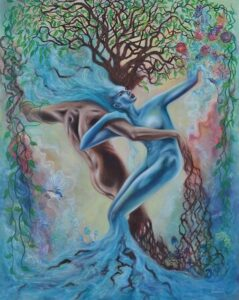
\includegraphics[width=.3\textwidth]{alchemical-marriage-image-5-239x300.jpg}
\end{wrapfigure}

Some midnight snacks for the contemplative.

\paragraph{Knowledge of the Heart}


\begin{quotex}
This direct perception of the truth, this intellectual and supra-rational intuition, a notion which the moderns seem to have lost, is truly ``knowledge of the heart'', to use an expression which is frequently encountered in Eastern doctrines. This knowledge is in itself something incommunicable; you have to have ``realized'' it, at least to some extent, to know what it really is; and all that can be said about it gives only a more or less approximate and inadequate idea. Above all, it would be a mistake to believe that one can actually understand what the kind of knowledge in question is when one is content to consider it ``philosophically'', that is to say from the outside, because we must never forget that philosophy is only a purely human or rational knowledge, as is all ``profane knowledge''.
\flright{\textsc{Rene Guenon}, \emph{Fundamental Symbols}}
\end{quotex}


When I was younger, I preferred philosophy of the grand type, like Spinoza or Francis Bradley. By a process of reasoning, beginning with the manifest world, they reached up to God (Spinoza) or the Absolute (Bradley). For the former, God is the sole Substance and, for the latter, the Absolute, the sole reality. Individuals therefore are less real.

On the level of profane philosophy, Ibn Arabi can be understood as the same type. For him God is Being, so beings are somehow less real. But Ibn Arabi is not doing philosophy but rather something far more profound. Following the Wisdom of Adam, there is the Manifest world. However, God Himself is Hidden, unlike the God of the philosophers. The True God can only be known through ``\emph{contemplation which is far from the results of thought}''. God reveals Himself as He sees fit and it is hubris to try to reach him solely through thought.

\paragraph{Anima Dreams}

Few men allow the Anima to roam freely. Rather they have distorted images of women in their mind. When they meet a real woman, they get confused. They say they can't figure her out, but that just means she does not fit into one of their categories. They don't know how to let go.

The quality of my Anima dreams has altered over the years. In one of the first that I recall, I was in the audience of a ``Reality'' show. The female hostess called me down to the stage, presumably to reveal reality to me; at that point I awakened.

In the next I dreamt of a woman asleep in a shallow creek, but water barely covering her. Clearly, I was awake in the scene, but the Anima was unconscious. The water is the symbol for the soul.

More recently, under the influence of another party, the Anima has been becoming more dominant. Just last week, I dreamed that I was asleep; I knew I was asleep although I had awareness. That sounds like being in the causal state.

Seated on a sofa a few meters away was a female figure, who seemed a little stiff. Some unseen person was asking her questions. When I realized that this Anima was taking over my soul and was speaking for me, I panicked and woke up screaming.

This path is not easy and can be threatening; otherwise it would be more common. The final dream will be the Alchemical Marriage.

\paragraph{World Cycles}


\begin{quotex}
The Krita Yuga Golden Age may well have been on ``earth'', but that does not necessarily imply that the earth itself was then what it is now; one could even wonder if it is not the changes of conditions which have occurred at certain times in the terrestrial world which prevent finding, by any research, truly ``primitive'' vestiges. --- I would say gladly also that ``on earth'' does not exactly mean ``on this earth''; the Islamic tradition speaks very clearly of the ``seven lands'', manifested successively or alternately, and which are moreover the same thing as the seven dvipas of the Hindu tradition. Of course, all this does not prevent considerations of origins in a more universal sense; but they must always be able, by appropriate transposition, to be applied at all levels, including that represented by the history of earthly humanity.
\flright{\textsc{Rene Guenon}, \emph{Letter to L C d'Amiens (22 April 1936)}}
\end{quotex}


Guenon provided precious few concrete details on the great cycles of Kalpas, Manvataras, and Yugas. In the letter above, he makes clear that these cannot be understood historically, archaeologically, nor scientifically. Rather they are states of being, and the ``Earth'' --- the planet we inhabit --- will differ from the Earth on another plane.

These cycles repeat each other. Eternal Lovers, or Polar Beings, chase each other across cycles or states of being. Situations and conditions repeat from one age to the next, with small variations. It is frustrating; it is exhilarating.

They may have to spend time wandering in a forest before they find each other. By then, karmic choices may weigh heavy on them, making their encounter all that much more difficult.

\paragraph{Devious Professions}


Some professions are inherently immoral because they are unnatural. For example, money is the medium of exchange. But to make it the product, as do the moneylenders, is what makes it unnatural.

Similarly, language is the medium of communications. But journalists, and similar professions, make it the product. Thus a writer may get paid by the word or by the size of the audience he attracts. That makes it immoral. True journalists, therefore, should be paid on the quality of their work, but there are very few of them.

The purpose of Law is to mediate between two disputants, not to take advantage of either party. There was a creepy skinny classmate from Tufts, who told me he wanted to become a divorce attorney because he thought he could get laid at a time when the women were feeling vulnerable. The next time, in a moment of weakness, you hold out any hope for the human race, keep that image in mind.


\flrightit{Posted on 2021-04-21 by Cologero}

\begin{center}* * *\end{center}

\begin{footnotesize}
\begin{sffamily}
\texttt{Santiago on 2021-04-26 at 21:01 said:}

``Seated on a sofa a few meters away was a female figure, who seemed a little stiff. Some unseen person was asking her questions. When I realized that this Anima was taking over my soul and was speaking for me, I panicked and woke up screaming.''

Why does this happen? It seems that the Anima, like the Absinthe green fairy, `wants your soul'. It ceases to be a figure worth romanticizing or lusting after, precisely at the moment when it becomes terrifying and domineering.

I think it tries to get us to confront certain things. I don't know why it does this, but I've noticed certain patterns, certain strategies it likes to employ for me. Yet, despite initially provoking me to lust, she will rarely if ever grant me control. I think she controls a good amount of the dream itself, to be honest. This may be why she got sloppy when you started to become lucid; her grasp on you and on the dream was rapidly slipping. Mine does similar things; the pretext of agency is gone and she fights for control and saps me of everything.

\hfill

\texttt{Cologero on 2021-04-29 at 07:52 said:}

Or else the Anima is your soul and She is demanding her rightful place in it.

\end{sffamily}
\end{footnotesize}

